\documentclass{standalone}
\usepackage{circuitikz}
\usepackage{schemabloc}

\begin{document}
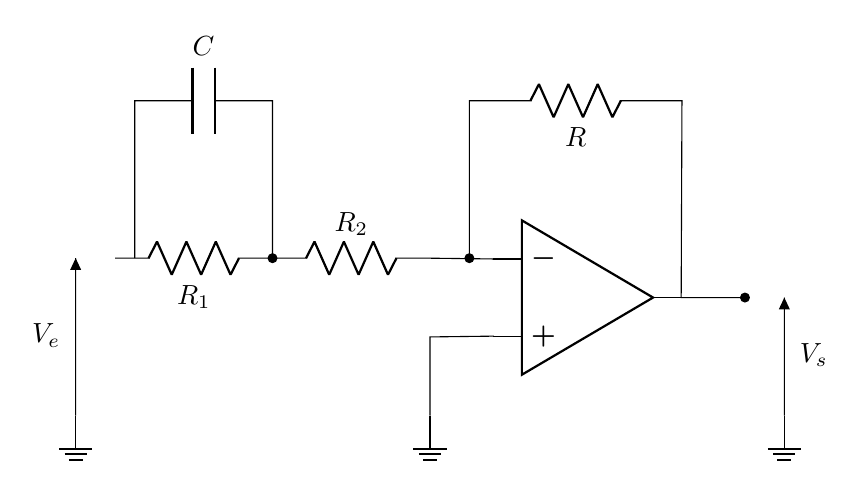
\begin{tikzpicture}

    \node[op amp, yscale=1] (opamp) at (6,-0.5) {};

    \draw (0,0) 
    to[R, l_=$R_1$,-] (2,0) 
    to[R, l=$R_2$, *-] (4,0) 
    to[short](opamp.-);

    \draw (0.25,0)
    to[short](0.25,2) 
    to[C, l=$C$,-] (2, 2) 
    to[short] (2,0);

    \draw (4.5,0) 
    to[short, *-] (4.5,2)
    to[R, l_=$R$,-] (7.2,2)
    to [short] (opamp.out)
    to [short, -*] (8, -0.5);

    \draw (opamp.+)
    to [short] (4, -1)
    to [short] (4, -2) node [ground] {};

    
    % closed 
    %input
    \draw (-0.5,0)
    to[short, l_=$V_{e}$](-0.5,-2)   node [ground] {};
    \draw (-0.5,0) coordinate[inputarrow,rotate=90];
    % output
    \draw (8.5,-0.5)
    to[short, l=$V_{s}$](8.5,-2)   node [ground] {};
    \draw (8.5,-0.5) coordinate[inputarrow,rotate=90];
\end{tikzpicture}
\end{document}